\documentclass[conference]{IEEEtran}
\usepackage[dvips]{graphicx}
\usepackage{amsfonts,epsfig,cite,array,url,ltablex,tabularx,setspace,arydshln,amssymb,multirow,multicol,mathptm,times,pstricks,subfigure}
\usepackage{threeparttable} 
\usepackage{ifpdf}
\usepackage{amsmath,epsfig,cite,graphicx,ltablex,tabularx,setspace,url,float,enumerate}
\usepackage[small,bf]{caption}
\renewcommand\captionfont{\scriptsize}
\usepackage{blindtext}
\usepackage{etoolbox}
\raggedbottom
\usepackage{multicol}
\usepackage{blindtext}
\interdisplaylinepenalty=2500

\begin{document}
\title{How Many Watts: A Data Driven Approach to Aggregated Residential Air-Conditioning Load Forecasting}

\author{\IEEEauthorblockN{Clement Lork\IEEEauthorrefmark{1}, Batchu Rajasekhar\IEEEauthorrefmark{2}, Chau Yuen\IEEEauthorrefmark{1}, Naran M. Pindoriya\IEEEauthorrefmark{2}}
	\IEEEauthorblockA{
		Engineering Product Development, Singapore University of Technology and Design, Singapore\IEEEauthorrefmark{1}\\
		Department of Electrical Engineering, Indian Institute of Technology Gandhinagar, India\IEEEauthorrefmark{2}\\
		Email: clement\_lork@mymail.sutd.edu.sg, batchu.rajasekhar@iitgn.ac.in, 
		yuen\_chau@sutd.edu.sg, naran@iitgn.ac.in}

}
\maketitle


\begin{abstract}
Due to the significant contribution of air-conditioning load towards total energy consumption in residential buildings, accurate modelling and forecasting of such load is key to effective demand-side energy management programmes. This paper suggests a data driven framework for 15 min-ahead AC load forecasting based on modern machine learning techniques that includes Support Vector Regression, Ensemble Trees, and Artificial Neural Network. To the end, it utilizes a correlation based feature selection method to identify information that is relevant for machine learning modelling. The effect of spatio-temporal features selection on prediction output and the effect of training data quantity on convergence characteristics were analysed and discussed. The effectiveness of the proposed approach is evaluated using a 20-household, half-year data set from an ongoing research testbed set up at the faculty housing units of Singapore University of Technology and Design. An linear combination method was proposed to combine models and the resulting model gave a mean absolute percentage error of 11.27\%. %This aggregated-home level prediction approach can be used by community energy manager to estimate the demand flexibility and participate in energy market on behalf of the customers.
\\
\end{abstract}
\begin{IEEEkeywords}
	Aggregate load forecasting, air-conditioning load, demand response, feature selection, machine learning, neural network, linear combination, and peak load shaving.
\end{IEEEkeywords}

\section{Introduction}
The development of the electricity grid in recent years has lead to an upgrade in internet communication technology between utilities and consumers. As part of this upgrade, the installation of smart meters and other home energy management systems bestows upon utilities sub-minute power consumption readings in real time, and fine control over specific appliances on the consumers' end. Policies developed on top of the upgraded infrastructure manipulate the usage of household appliances to achieve energy savings and efficiency\cite{li2014}. Of all the appliances in modern homes, an interesting appliance to note is the air-conditioning (AC) system. ACs are well suited to provide demand reduction, load following, and regulation services, as they could be turned off or reduced for short period without much discomfort to the consumers. Not only are ACs ubiquitous in modern residences, they can amount to an average of 45\% of residential electricity consumption\cite{kalkan2012}. Since ACs forms such a major portion of customers electricity demand, AC control mechanisms that help to reduce energy usage benefits both customers and utilities\cite{Yoon2016,PacificGasandElectricCompany,peaksaver}.

Before the implementation of any AC control mechanism, there is a need to quantify and forecast the amount of energy that can be shifted or reduced by the control event. The introduction of highly stochastic renewable generation and dynamic pricing in the electricity market has led to more frequent fluctuations in the state of the electricity market. This has driven up the need for AC forecasting models to predict ahead for a short interval of between 5 mins to 30 mins, to keep up with the fluctuations in market conditions\cite{Chan2012}. Thus, the focus of this paper is to suggest a framework to forecast AC load within the short time frame. 
\subsection{Related Works}
  AC energy consumption modelling can be classified into three distinctive categories: whitebox/engineering models, blackbox/statistical based models, and grey-box models. All these models try to forecast AC load as a function of several variables. The engineering models attempt to derive the energy consumption of an AC compressor based on a physical model of the thermal characteristics of the residence\cite{zhang2013}. Since the thermal characteristics includes furniture placement and occupancy behaviour, it is difficult to obtain exact measurements for each residence in real life, resulting in inaccuracies. Black box models use either statistical or machine learning methods to fit a functional model of AC load based on historical load conditions and other variables at hand. Although it is the easiest to implement, model parameters have to be carefully chosen to avoid the garbage in-garbage out phenomenon. Some examples of black box models include a stochastic tobit model\cite{Horowitz2014}, a machine learning SVR model\cite{xuan2015}, and a hybrid stochastic/machine-learning model with ARIMA and BPNN\cite{xuemei2009}. Grey box models combine physical functions with parameters estimated by statistical or machine-learning means. Difficulty in implementing grey box model depends on the getting the physical functions right, which could be complex at times. A forecast of non inverter AC load was attempted by estimating the thermal conditions of residential rooms  via linear regression and linking it with a thermal model\cite{jain2016}. In AC modelling scenarios, knowledge of physical characteristics of the system is seldom complete. Black box modelling is best suited for modelling AC load as it does not require any prior knowledge on the system. Moreover, it can capture the complex dynamics between the variables, and is chosen to be the focus of this research.
   
 \subsection{Contributions}
  Since the black box modelling approach does not assume any knowledge of the system, we will have to discover what are the inputs that are most impactful in modelling, and which featureset corresponds to which black box modelling technique for best performance. This paper intends to encapture this discovery process as simple black box modelling framework, in order to select the best model for AC load forecasting and modelling with real world data. This is unlike most of the papers surveyed, which directly appoint a set of predefined featuresets and modelling techniques. Those models have low modelling intervals of 30 min or longer, leading to loss in information on demand variations, and hampering control requiring high resolution inputs. Also, they do not study the operating parameter settings on overall load variations but focuses just on historical load and weather data.
  Here we:     
\begin{itemize}
	\item Derived additional variables from our dataset which includes load, weather and AC operational parameters, apart from just using load and weather data. From these variables, we identify the minimal viable featuresets.
	\item Studied popular machine learning methods with a short 15-min modelling interval, and quantify number of training samples and input featuresets for best performance of each technique. 
	\item Proposed a linear combination method to search for the optimal combinatory model
\end{itemize}
The resulting framework can be adopted by aggregators to forecast and predict AC demand potential for other AC datasets. The remainder of the paper is organized as follows: Section. \ref{frame} briefly describes the modelling framework, Section. \ref{dataproc}-\ref{mcom}, discusses an application of the framework real world data, and finally Section. \ref{conc} wraps up with the observations and future scope.

\section{Framework}\label{frame}
In this framework, there are four steps as shown in Fig.\ref{framework}.
Within each step, techniques like modelling techniques or data cleaning techniques are means to accomplish a task and are interchangeable.
\begin{figure}[htb!]\centering \footnotesize
	\includegraphics[width=75mm]{Framework1}
	\caption{Framework for Load Forecasting}
	\label{framework}
\end{figure} 
\subsection{Data Processing}
Dataset often contains missing or erroneous data. Depending on the amount of data that are missing, different techniques could be used\cite{cleophas2016}. To patch up the dataset, a matlab script was written to identify missing and erroneous data, before performing linear interpolation. All datatypes are also synced to the same time frame. Derived features deemed to affect predictions are also generated. The impact of the derived features are estimated in the next step of featureset generation.
\subsection{Featureset Generation} 
Inputs for black box models are pivotal for prediction accuracy. A model trying to draw relationship from too many variables struggles to extract signal from noise, resulting in poor performance. Therefore it is imperative to select the right featureset. Historical data are known to affect prediction accuracy, but how far should we look back to? In order to solve this, we ranked the features according to Pearson Correlation Coefficient (PCC), examine the PCC of lagged consumption values and decide the maximum amount of time lag we afford to the featureset.
\subsection{Model Selection}
Each modelling technique possesses different tunable parameters and sensitivity towards the input featureset. A model consists of the technique together with it's input featureset. Here, we hold the tunable parameters of each modelling technique constant and only vary the input featureset for each technique. five-fold cross validation\cite{zhang1993} was implemented to identify the best model across the three techniques to avoid biases.  

\subsection{Model Combination}
 Even if a model does not provide the best accuracy, it still contain useful information. Some models overpredict, some models underpredict. By combining different models together, their inaccuracies will be averaged out and a stronger predictor might emerge\cite{dvzeroski2004}. After selecting the best model for each technique, we check the combinatory affinity of the three models via a customized linear optimization process. 
 
 \section{Data Processing} \label{dataproc}
 A wireless sensor network testbed is setup in the faculty housing apartments at Singapore University of Technology and Design (SUTD). This testbed  has a total of 20 homes with 68 Panasonic inverter ACs, supported by 36 compressors (CU-S24PKZ). Weather data is obtained from a local weather station in SUTD.

The buildings testbed data consists of individual AC system operating parameters and power consumption values for 20 homes measured for a period of 275 days (1 April 2015-31 December 2015), sampled at every 30 seconds. The appropriate weather data set is matched to the building data set via common time stamps to form a single data set. For the dataset, there are erroneous values, and missing values due to communication delays and losses between the data collection hardware and the server. When the erroneous and missings value happen within a 15 mins period, a linear interpolation technique was applied, where these values are replaced by the averaged series of the non-erroneous values from before and after each erroneous event. Since the interest is in 15 minutes ahead load prediction, the data set is down sampled from a period of 30 seconds into one of 15 minutes by taking the average of 30 half-min data within each 15 minutes block. Even after interpolation, the region between 8 Jun 2015 to 15 Jun 2015 has an unnaturally low region of power consumption, due to a huge chunk of missing data. Hence, to preserve the integrity of the data used for investigation, data were taken from 1 Jul 2015 to 31 Dec 2015, for a total of 184 days, and the rest discarded. The month of August 2015 was separated out as the test set, while the months of July 2015, September to December 2015 were considered the training set. The day type of each day were encoded according to the Singapore 2015 calender where Public holidays are considered as Sundays and each day is given a numerical label 1 through 7 in ascending order with Sunday being 1. Meanwhile, the $'$ON$'$ and $'$OFF$'$ operating states were denoted with a binary variable.

\begin{table}[H]
	\centering
	\caption{Feature List}\label{features}
	\resizebox{88mm}{!}{
		\label{featuredescription}
		\begin{tabular}{@{}ll@{}}
			\hline
			\textbf{Feature name} & \textbf{Feature Description} \\\hline
			Time ($T$) & 1 to 96 each for each 15 min blocks in a day \\
			Daytype ($D$) & 0 for weekdays, 1 for weekends and public holidays \\
			Outdoor Temp ($OTemp$) & Measured from weather station \\
			Heat Index ($HI$) & \begin{tabular}[c]{@{}l@{}}Measured from weather station, a metric that takes into \\ account humidity and temperature\end{tabular} \\
			Wind Chill ($WC$) & \begin{tabular}[c]{@{}l@{}}Measured from weather station, a metric that takes into \\ account temperature and wind speed\end{tabular} \\
			Desired Temp ($DTemp$) & \begin{tabular}[c]{@{}l@{}}Averaged AC temperature set point for all users at a certain \\ time\end{tabular} \\
			Desired Temp On ($DTempOn$) & Averaged AC set point for all users that have AC on \\
			Indoor Temp ($ITemp$) & Averaged indoor temp for all user measured by the AC \\
			Indoor Temp On ($ITempOn$) & \begin{tabular}[c]{@{}l@{}}Averaged indoor temp for all user measured by the AC , \\ while AC is on\end{tabular} \\
			Total Status ($S$) & No of compressors switched ON at a certain time \\
			Total Power Consumption ($P$) & Total AC consumption \\
			Power Change ($PC$) & Difference of power consumption in two intervals, $P(t)-P(t-1)$ \\
			Status Change ($SC$) & Difference of Total Status in two intervals, $S(t)-S(t-1)$\\ \hline
		\end{tabular}
	}
\end{table}
The list of features in the dataset and their description are summarized in Table. \ref{features} above. The original dataset after data cleaning and encoding consist of 9 features, Time($T$), DayType($D$), Outdoor Temp($OTemp$), Heat Index($HI$), Wind Chill($WC$), Desired Temperature($DTemp$), Indoor Temperature($ITemp$), Total Status($S$), and Total Power($P$). Derived features were added to draw an improved relationship between variables and power consumption. 
$DTemp$, and $ITemp$ were read off the AC controller of each room and the AC could be either ON or OFF. However, logically, only the $DTemp$, and $ITemp$ of ACs that are switched on will affect the power consumption. Therefore, $DTempOn$, and $ITempOn$ were generated by summing up all the $DTemp$, and $Itemp$ of AC that are switched On divided by the total number of AC, which is 68. Power Change($PC$), and Status Change($SC$) were generated by taking the difference between the current $P$, $S$ value, and the value one time step before. This is to characterize the operating transient of the ACs. When a single AC is switch ON from OFF, there will be a spike in the power that it draws and then decrease as the room cools. A change in $SC$ will be reflected in the change in $PC$. $T$ and $D$ are categorical variables and are always considered in generating models. $OTemp$, $HI$, $WC$, $DTemp$, $DTempOn$, $ITemp$, $ITempOn$, $S$, $P$, $PC$, $SC$ are time series variables. The time series variables are considered to be in a feature set $F$ and are further investigated in the next section. 

\section{Featureset Generation}\label{fgen}
 There are generally two ways of selecting features, filter or wrapper based. Filter based techniques consist of passing input features through an evaluation criteria like Mutual Information, RReliefF or even just Pearson Correlation Coefficient to rank their importance to the variable to be modeled. Wrapper techniques are more complex as they require input features to be parsed by a forecasting model and the resulting prediction accuracy fed back as a evaluation criteria to rank the features. A particular work on electrical load forecasting \cite{Hu201517} hybridized the two different classes of feature selection method to form a feature selection pipeline. For the sake of streamlining the feature inputs, we used a filter method via Pearson Correlation Coefficient (PCC) to select a subset of features $F_{sel}$ from the set of features $F$ in the original dataset. Then, we will evaluate the amount of lag to be given to $F_{sel}$ based on correlation analysis of lagged power consumption values. 
\subsection{Pearson Correlation Analysis}
\begin{equation}
\footnotesize
\rho (A,B) = \frac{1}{{N - 1}}\sum\limits_{i = 1}^N {\left( {\frac{{\overline {{A_i} - {\mu _A}} }}{{{\sigma _A}}}} \right)} \left( {\frac{{\overline {{B_i} - {\mu _B}} }}{{{\sigma _B}}}} \right)
\label{PCC}
\end{equation}
The equation to PCC is shown in (\ref{PCC}). Here, $\mu_A$ and $\mu_B$ are the mean of variables $A$ and $B$ respectively, while $\sigma_A$ and $\sigma_B$ are the standard deviation of $A$ and $B$ respectively. The PCC can range from -1 to 1, with 1 representing complete positive correlation, and -1 representing complete negative correlation. For this paper, the absolute value of the correlation is considered. Within the original dataset, $T$ and $D$ are categorical variables and are not considered in the correlation analysis. $P$ is the variable to be forecasted and is assigned as variable $A$ in the PCC. The remaining feature $OTemp$, $HI$, $WC$, $DTemp$, $DTempOn$, $ITemp$, $ITempON$, $S$, $PC$ and $SC$ are assigned to be $B$, and PCC is calculated for each feature. 
\begin{table}[htb!]
	\centering
	\caption{Pearson Coefficient Analysis of Various Features against Power Consumption}
	\label{correlationtable}
	\resizebox{70mm}{!}{
		\begin{tabular}{@{}lllll@{}}
			\hline
			\textbf{\textit{ITempOn}} & \textbf{\textit{S}} & \textbf{\textit{DTempOn}} & \textbf{\textit{SC}} & \textbf{\textit{PC}} \\ \hline
			0.5809 & 0.5680 & 0.5366 & 0.2063 & 0.2054 \\ \hline
			\textbf{\textit{DTemp}} & \textbf{\textit{HI}} & \textbf{\textit{OTemp}} & \textbf{\textit{WC}} & \textbf{\textit{ITemp}} \\ \hline
			0.1623 & 0.1529 & 0.1004 & 0.1004 & 0.0922 \\ \hline
		\end{tabular}
	}
\end{table}
As displayed in Table. \ref{correlationtable}, the top 5 features are \textit{ITempOn}, \textit{S}, \textit{DTempOn}, \textit{SC}, and \textit{} with a PCC value of more than 0.2, signifying some linear relationship with $P$. For variables with PCC under 0.2, they do not affect power consumption much, as seen in Fig. \ref{boxplot}, a boxplot of the features against $P$. Most of these variables below the threshold are exogenous weather variables. The values above the PCC threshold of 0.2 are selected to be part of $F_{sel}$. $F_{sel}$ will be tested against against a set of all features, $F_{all}$ , during the model selection process in order to determine the effectiveness of the feature selection process.  
\begin{figure}[htb!]\centering \footnotesize\vspace{-1em}
	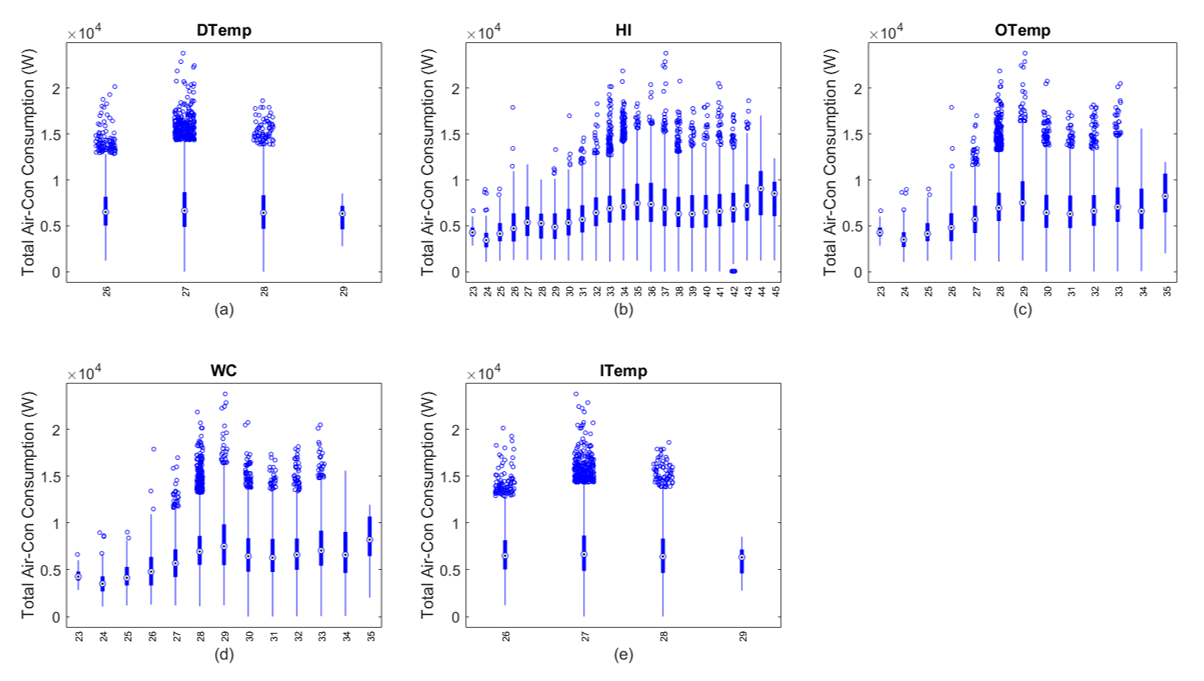
\includegraphics[width=88mm]{boxplots}
	\caption{Boxplots of features against P with PCC under 0.2}
	\label{boxplot}
\end{figure}

	
\subsection{Lagged Feature set Generation}
\begin{figure}[htb!]\centering \footnotesize\vspace{-2em}
	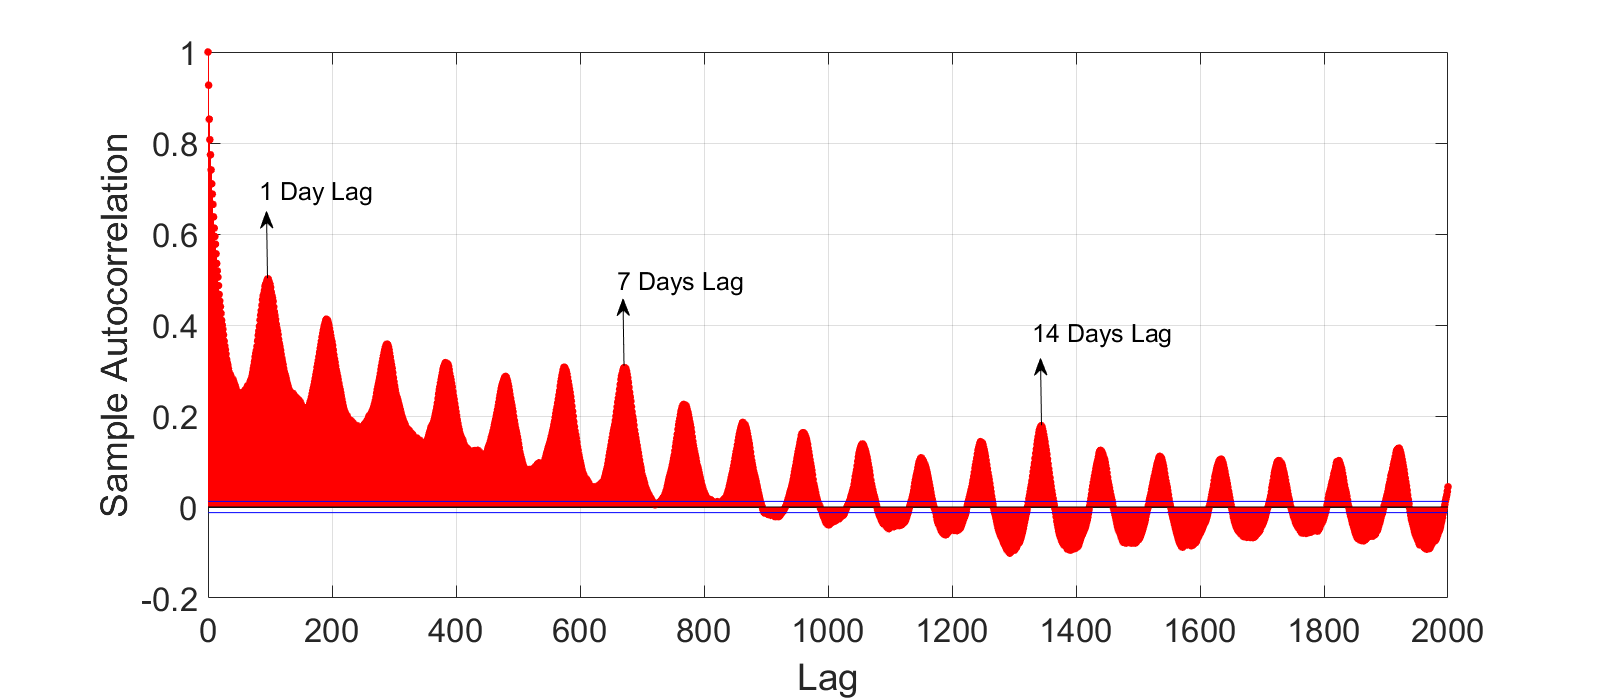
\includegraphics[width=88mm]{correlationfunctioneditted}
	\caption{Correlation of Power Consumption with its Lagged Series}
	\label{correlationfunction}
\end{figure}
The PCC relationship between lagged \textit{P} values and \textit{P} could be seen in Fig. \ref{correlationfunction}. The lagged variables nearest to the original time showed the highest correlation to the power consumption, and decrease until another peak at the same time of the previous day $(t-96)$, and then another peak at same time of the previous week $(t-672)$ and so on. These peaks signify the important lag points that should be taken when lagging the feature set. Lagging $P$ beyond the third week $(t-1344)$ shows a PCC of below 0.2. The third week forms the lower bound for lagged P values. A few combination of lag values before 1344 were selected to be compared between different machine learning models and could be seen in Table. \ref{performstats}. The variables to be lagged are $P$, $ITempOn$, $S$, $DTempOn$, $SC$ and $PC$. After the variables are lagged by the respective amount, the set is appended with the $T$ and $D$ variables to form the complete feature set as listed in Table. \ref{performstats} under the column features. For example 'Selected(1:4)' is a feature set containing $T$, $D$, $P(t-1)$, $ITempOn(t-1)$, $S(t-1)$, $DTempOn(t-1)$, $SC(t-1)$, $PC(t-1)$, $P(t-2)$, $ITempOn(t-2)$, $S(t-2)$, $DTempOn(t-2)$, $SC(t-2)$, $PC(t-2)$... $P(t-4)$, $ITempOn(t-4)$, $S(t-4)$, $DTempOn(t-4)$, $SC(t-4)$, $PC(t-4)$. For the feature set label 'All', features includes $T$, $D$ and lagged variables of $P$, $ITempOn$, $S$, $DTempOn$, $SC$, $PC$, $DTemp$, $HI$, $OTemp$, $WC$, and $Itemp$.

\section{Model Selection}\label{msel}
The machine learning models that are used contains several tunable parameters. These parameters are held constant as we are interested in validating the feature selection process.
\subsection{Machine Learning Models}
\subsubsection{Support Vector Regression (SVR)}
The SVR aims to find an optimal hyperplane that can describe $P$ from the feature set $F$\cite{basak2007}. The parameters to be tuned are the cost of the error $C$, the margin for error $\epsilon$ and the kernel function $\Phi$. $C$ and $\epsilon$ are set at the standard deviation of $P$ during the training to account for outliers. $\Phi$ is the Gaussian kernel to handle the non-linearity relationships between variables.  
\subsubsection{Ensemble Trees (ET)}
ET is a combination of single layer decision trees that discretize the functional space between $P$ and $F$ to make predictions. The training method is selected to be LSBoost\cite{friedman2001} and the parameters selected are the number of tree, $n$=100 and the learning rate $\eta$=0.1
\subsubsection{Artificial Neural Network (ANN)}
The ANN used is a 3 layered feed forward perceptron. The featureset $F$ is connected to a hidden layer of nodes and the hidden layer leads to the output prediction of $P$. The training method to find the weights of each connection is selected to be the Levenberg-Marquardt\cite{yu2011} method and the number of nodes in the hidden layer is $n$=10. The transfer function in the hidden layer is the sigmoid function while the transfer function in the output layer is the linear function.

\subsection{Investigation of input features on different machine learning methods}
\begin{table}[H]
	\resizebox{88mm}{!}{
		\centering
		\begin{threeparttable}[b]
			\caption{Performance statistics of SVR, ET, and ANN models for day-ahead forecasting}
			\label{performstats}
			\def\arraystretch{1.2}% 
			\begin{tabular}{|l|l|l|l|l|l|l|}
				\hline
				\multirow{2}{*}{Features}                                              & \multicolumn{3}{c|}{RMSE (watts)}                                                 & \multicolumn{3}{c|}{MAPE }                                                   \\ \cline{2-7} 
				& SVR    & \begin{tabular}[c]{@{}l@{}} ET \end{tabular} & ANN    & SVR     & \begin{tabular}[c]{@{}l@{}} ET \end{tabular} & ANN     \\ \hline
				Selected (1:4)                                                         & 1243.7 & 1090.6                                                  & 1066.2 & 0.7734  & 0.4885                                                  & 0.3159  \\ \hline
				All (1:4)                                                              & 1280.7 & 1089.9                                                  & 1070.2 & 0.8573  & 0.5042                                                  & 0.2425  \\ \hline
				Selected (1:8)                                                         & 1272.2 & 1089                                                    & 1067.2 & 0.5973  & 0.5033                                                  & 0.2477* \\ \hline
				All (1:8)                                                              & 1306   & 1088.4                                                  & 1078.5 & 0.6501  & 0.5125                                                  & 0.2979  \\ \hline
				\begin{tabular}[c]{@{}l@{}}Selected (1:12)\end{tabular}            & 1279.5 & 1089                                                    & 1082.8 & 0.6067  & 0.5020*                                                 & 0.3077  \\ \hline
				All (1:12)                                                             & 1306.2 & 1088.7                                                  & 1102.7 & 0.6372  & 0.508                                                   & 0.3064  \\ \hline
				\begin{tabular}[c]{@{}l@{}}Selected (1:8,96)\end{tabular}          & 1247.2 & 10883                                                   & 1086.9 & 0.5679  & 0.5109                                                  & 0.2591  \\ \hline
				All (1:8,96)                                                           & 1278.9 & 1088.1                                                  & 1095.2 & 0.6099  & 0.5162                                                  & 0.2829  \\ \hline
				\begin{tabular}[c]{@{}l@{}}Selected (1:8,96:104)\end{tabular}      & 1270.2 & 10885                                                   & 1108   & 0.4342* & 0.5108                                                  & 0.3099  \\ \hline
				\begin{tabular}[c]{@{}l@{}}All (1:8,96:104)\end{tabular}           & 1296   & 1088.1                                                  & 1182.8 & 0.4614  & 0.5148                                                  & 0.3337  \\ \hline
				\begin{tabular}[c]{@{}l@{}}Selected (1:8,96,672)\end{tabular}      & 1233.2 & 1088.6                                                  & 1131.6 & 0.4764  & 0.511                                                   & 0.2535  \\ \hline
				\begin{tabular}[c]{@{}l@{}}All (1:8,96,672)\end{tabular}           & 1260.8 & 1088.2                                                  & 1105.5 & 0.4994  & 0.5162                                                  & 0.3372  \\ \hline
				\begin{tabular}[c]{@{}l@{}}Selected (1:8,96,672,1344)\end{tabular} & 1222.8 & 1088.7                                                  & 1081.5 & 0.4406  & 0.5128                                                  & 0.275   \\ \hline
				\begin{tabular}[c]{@{}l@{}}All (1:8,96,672,1344)\end{tabular}      & 1249.4 & 1088.1                                                  & 1153   & 0.4632  & 0.5161                                                  & 0.3508  \\ \hline
				\end{tabular}
				\begin{tablenotes}
					\item[1] $*$indicates selected models for final prediction
					\end{tablenotes}
					\end{threeparttable}
					}
					\end{table}
					
Root Mean Square Error (RMSE) and Mean Absolute Percentage Error (MAPE) are usually used as quality measures. The RMSE described in (\ref{eqn9}) is used as error measure to evaluate the results.
\begin{equation}
\footnotesize
RMSE = \sqrt {\frac{1}{N}{{\sum\limits_{t = 1}^N {\left[ {\left( {{P_{real}}(t) - {P_{estimated}}(t)} \right)} \right]} }^2}}
\label{eqn9}
\end{equation}
where, ${{P_{real}}(t)}$ and ${{P_{estimated}}(t)}$ are real and forecast power consumption respectively. MAPE is used to compare performance on different data sets, as it is a relative measure. The MAPE described in (\ref{eqn10}) is used to evaluate the forecasted results, as it will be less skewed towards outliers than RMSE.
\begin{equation}
\footnotesize
MAPE = 100 * \frac{1}{N}\sum\limits_{t = 1}^N {\left| {\frac{{{P_{real}}(t) - {P_{estimated}}(t)}}{{{P_{real}}(t)}}} \right|} 
\label{eqn10}
\end{equation}					
					
For each model using different input combinations mentioned, 5 fold cross-validations are carried out on the training set. The performance statistics of three models are given in Table \ref{performstats}. By looking at the MAPE value, ANN has shown to have a much lower error than the rest of the machine learning methods. If a single model is to be chosen, ANN could be ideal. Generally, the model will perform better with the selected variables as compared to using all the variables as quantified by the MAPE value. Different models have different tolerances for the amount of lagged inputs. For the selected featureset, ANN generally requires 1:8 lags to perform well, as compared to ET which requires 1:12 lags. SVR requires the most amount of data, requiring inputs with 1:8, 96:104 lags. The best models selected for the next set of investigation are highlighted with the symbol $*$ in Table \ref{performstats}.
					
\subsection{Investigation of training samples on each model}
The three selected models were then tested with the test data from the month of August 2015 and trained with all the training data from the month of July 2015 and from September to December 2015. Training data were divided randomly into chunks of 500 data points and then fed into the model to test the learning sensitivity of the models. The results are summarized in Fig. \ref{learningpotentialedited} below. 
\begin{figure}[htb!]\centering \footnotesize
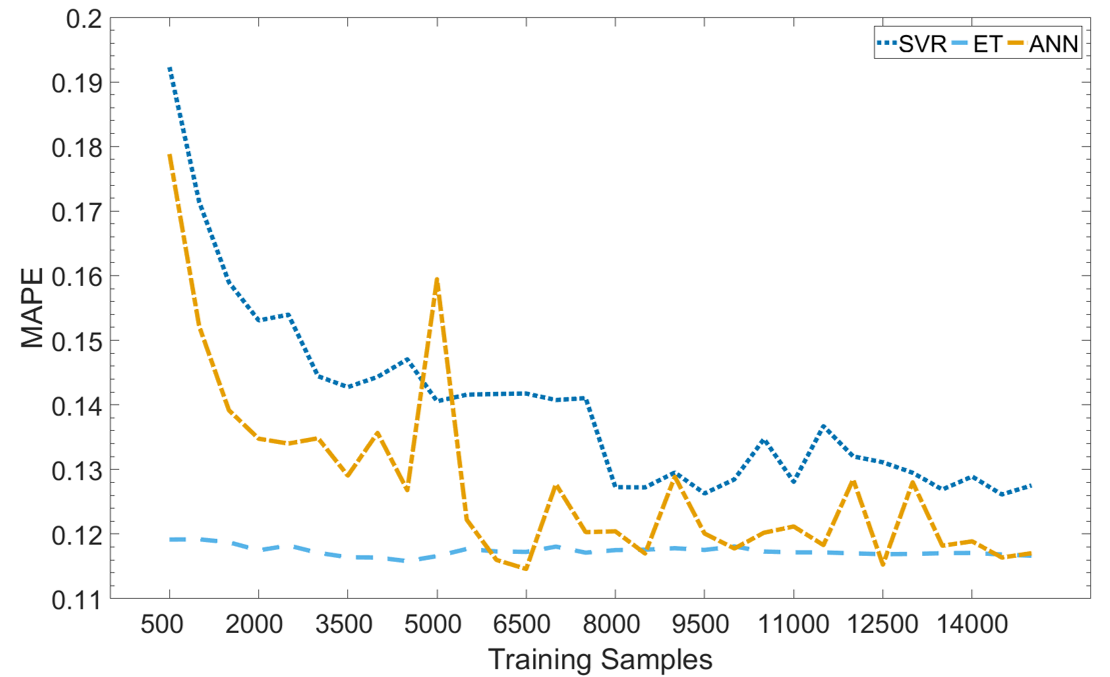
\includegraphics[width=80mm]{learningpotentialforecasting}
\caption{Learning Curves for Selected Models}
\vspace{-0.3cm}
\label{learningpotentialedited}
\end{figure}
From the plots, ET has shown to require the least amount of data to reach the minimum MAPE. In fact, it could be trained with just 500 data points, which amounts roughly to a week's worth of data. Comparatively, ANN requires some 6500 data points and SVR requires 8000, 10 weeks and 12 weeks worth of data respectively. In a day to day scenario, where a smart meter is required to make forecasts from limited data, ET could be deployed as a first layer predictor, supported by the ANN and ET predictors when there is more data available.  
						
\section{Model Combination}\label{mcom}

\subsection{Proposed hybrid methodology}
The final training results for 15min ahead forecasting are displayed in Fig. \ref{wholetestset} and Fig. \ref{dayprediction}. Fig. \ref{wholetestset} showcased the predictions for two weeks of the entire month. For the most part, the prediction models are able to capture the dynamic AC load pattern and give accurate predictions.   
\begin{figure}[htb!]\centering \footnotesize
	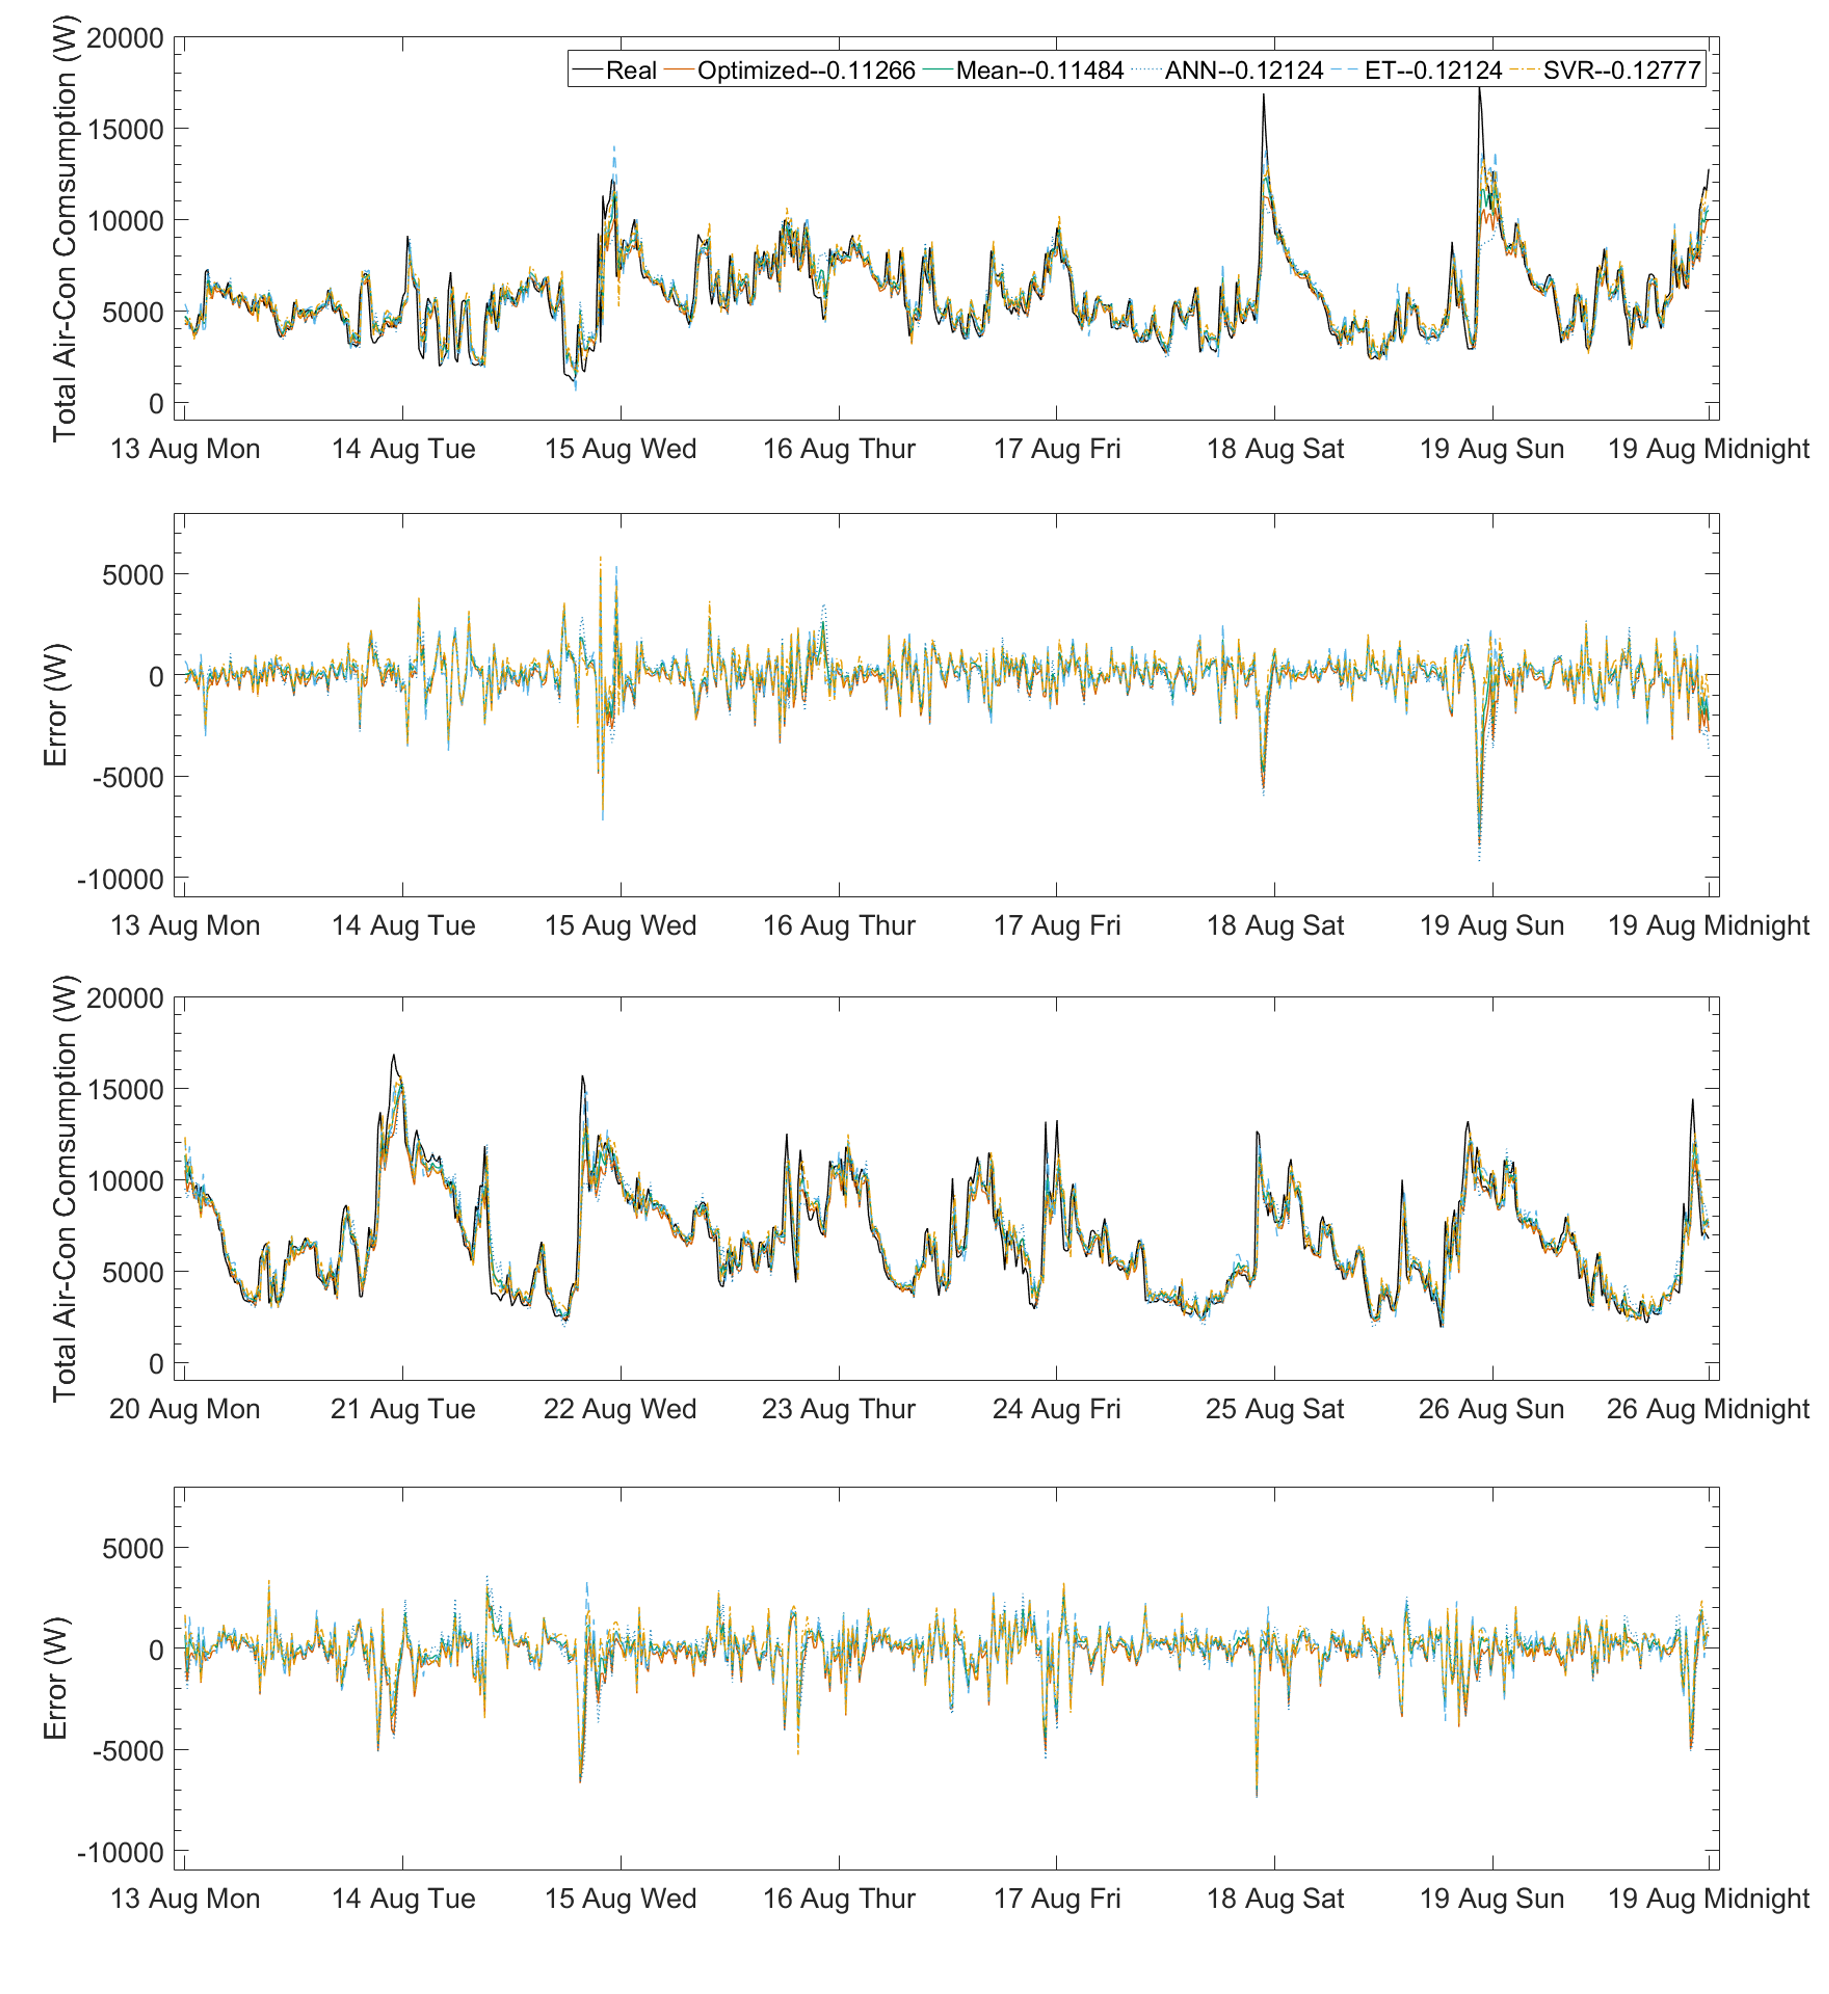
\includegraphics[width=88mm]{2weeks}
	\caption{Prediction Plot from 13 August to 26 August, 2015}
	\vspace{-0.3cm}
	\label{wholetestset}
\end{figure}
 The prediction accuracy is 0.12777 for SVR, 0.12124 for ET and 0.12124 for ANN over the entire month of August 2015.
 \begin{figure}[htb!]\centering \footnotesize
 	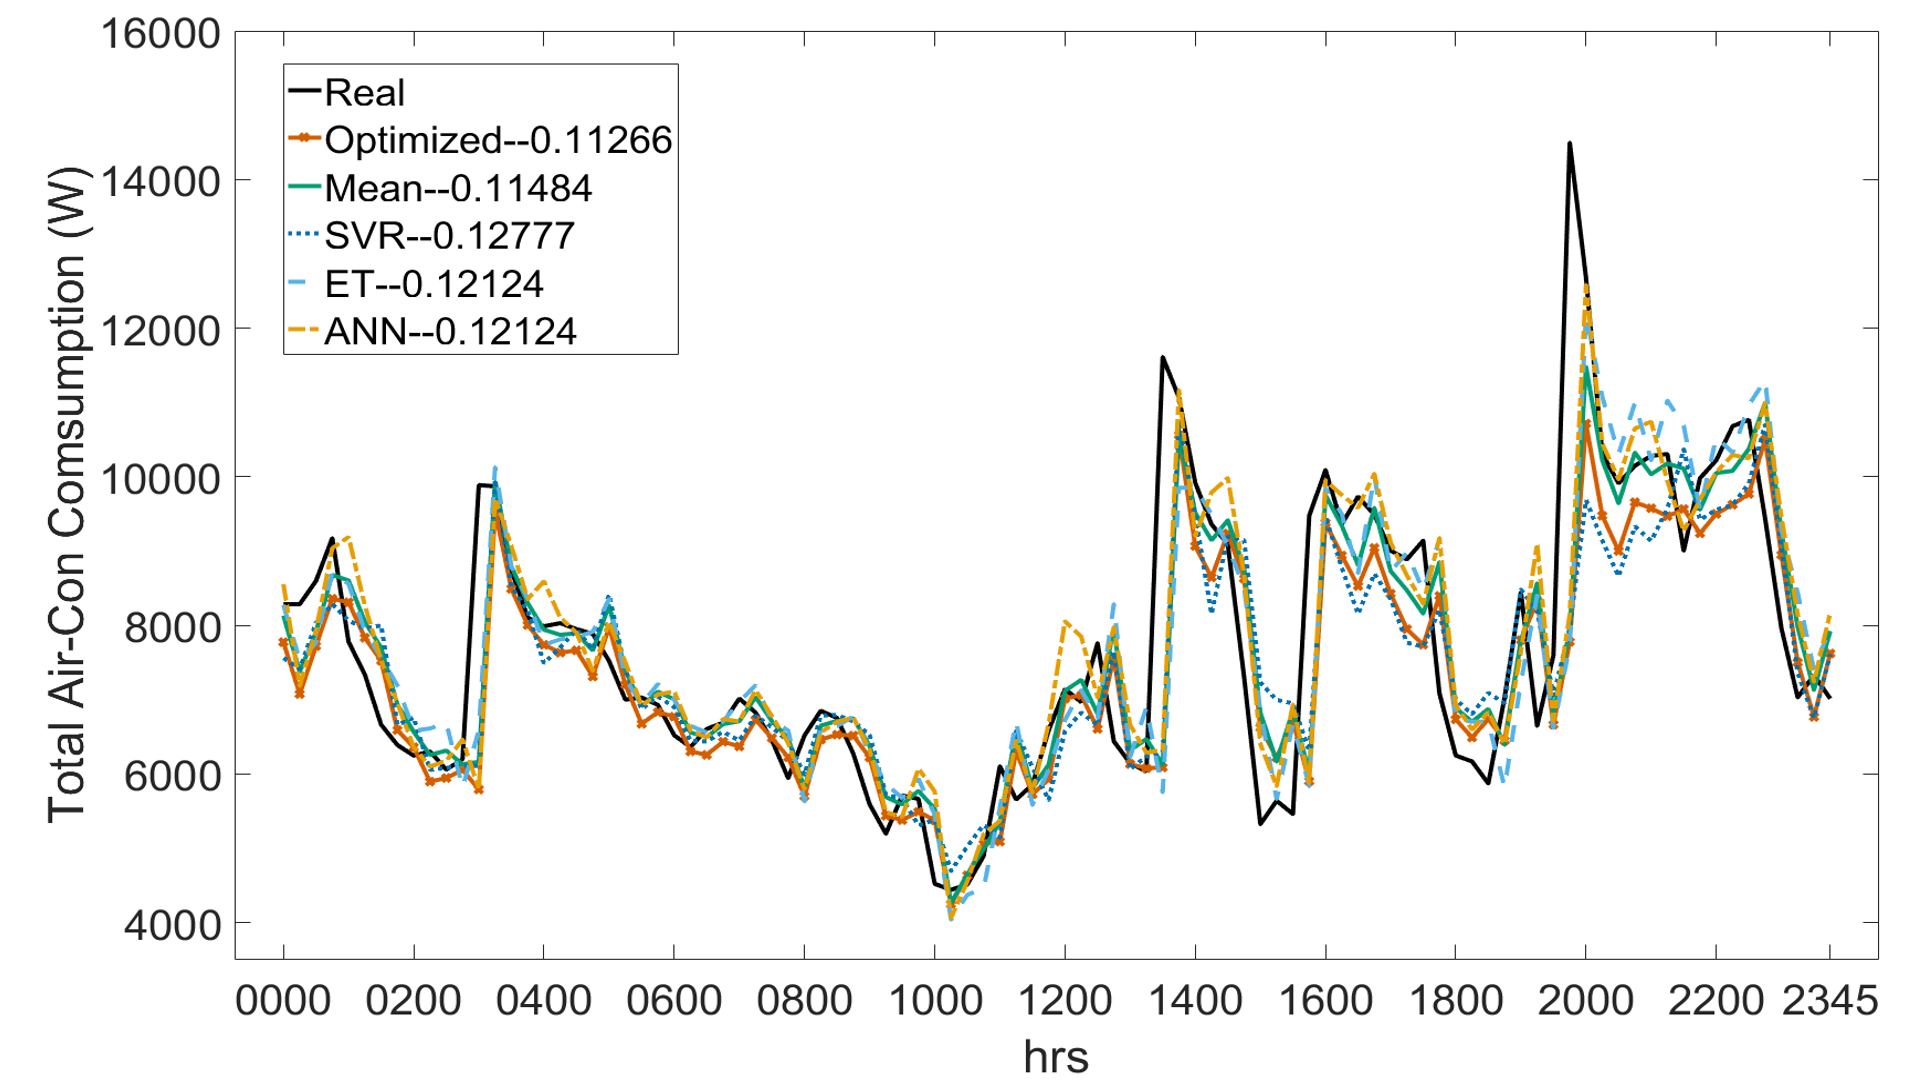
\includegraphics[width=80mm]{prediction}
 	\caption{Prediction for 1 August 2015}
 	\vspace{-0.3cm}
 	\label{dayprediction}
 \end{figure}
  Notice in the prediction plots for 1 August 2015 in Fig. \ref{dayprediction}, SVR as represented by the dark blue line, is mostly outputting values that are lower than the real outputs as represented by the black line. Meanwhile, ANN and ET, represented by the orange and light blue lines respectively, have values that are above the black line. Rather than simply averaging the three models to improve accuracy \cite{lan2009}, a linear optimization problem is formulated.
We are interested in finding a scaling coefficient to the models during the training period such that the linear combination of the models with their respective $F_{sel}$ will approximate the $P$ of the training set, but not \textbf{equals} to the $P$ of the training set. This is to avoid overfitting on the training set which will result in poor performance on the test set.  
\begin{equation}
\footnotesize
	a_1SVM(F_{sel,SVR}^{train})+a_2ET(F_{sel,ET}^{train})+a_3ANN(F_{sel,ANN}^{train}) = MDL^{train}
\end{equation}
To avoid overfitting, we introduced a constraint to not take outliers into account. Outliers in this case are defined as 3$\sigma$ away from the mean of $P^{train}$.
\begin{equation} \label{minimization}
\footnotesize
\begin{aligned}
&\min_{a_1,a_2,a_3} (MDL^{train}-P^{train})^2\\
& \text{subject to:}\\
&a_1SVM(F_{sel,SVR}^{train})+a_2ET(F_{sel,ET}^{train})+a_3ANN(F_{sel,ANN}^{train})\\ 
&\leq mean(P^{train})+|3\sigma|
\end{aligned}
\end{equation}
Solving (\ref{minimization}) gives $[a_1, a_2, a_3]$ of [0.5000,0.0314,0.4363] and when these coefficients were applied to predicting the test set, $MDL^{test}$ gave an MAPE of 0.11266. This is a better result than simply averaging the three models\cite{lan2009} which gives an MAPE of 0.11484. The optimized model is shown as the red line in Fig. \ref{wholetestset} and \ref{dayprediction}, while the mean of models shown is as the green line. The optimized model predicts better than purely SVR, ET and ANN as it contains less percentage error of higher magnitudes as shown in the error histograms of Fig. \ref{errorhist}
 \begin{figure}[htb!]\centering \footnotesize
 	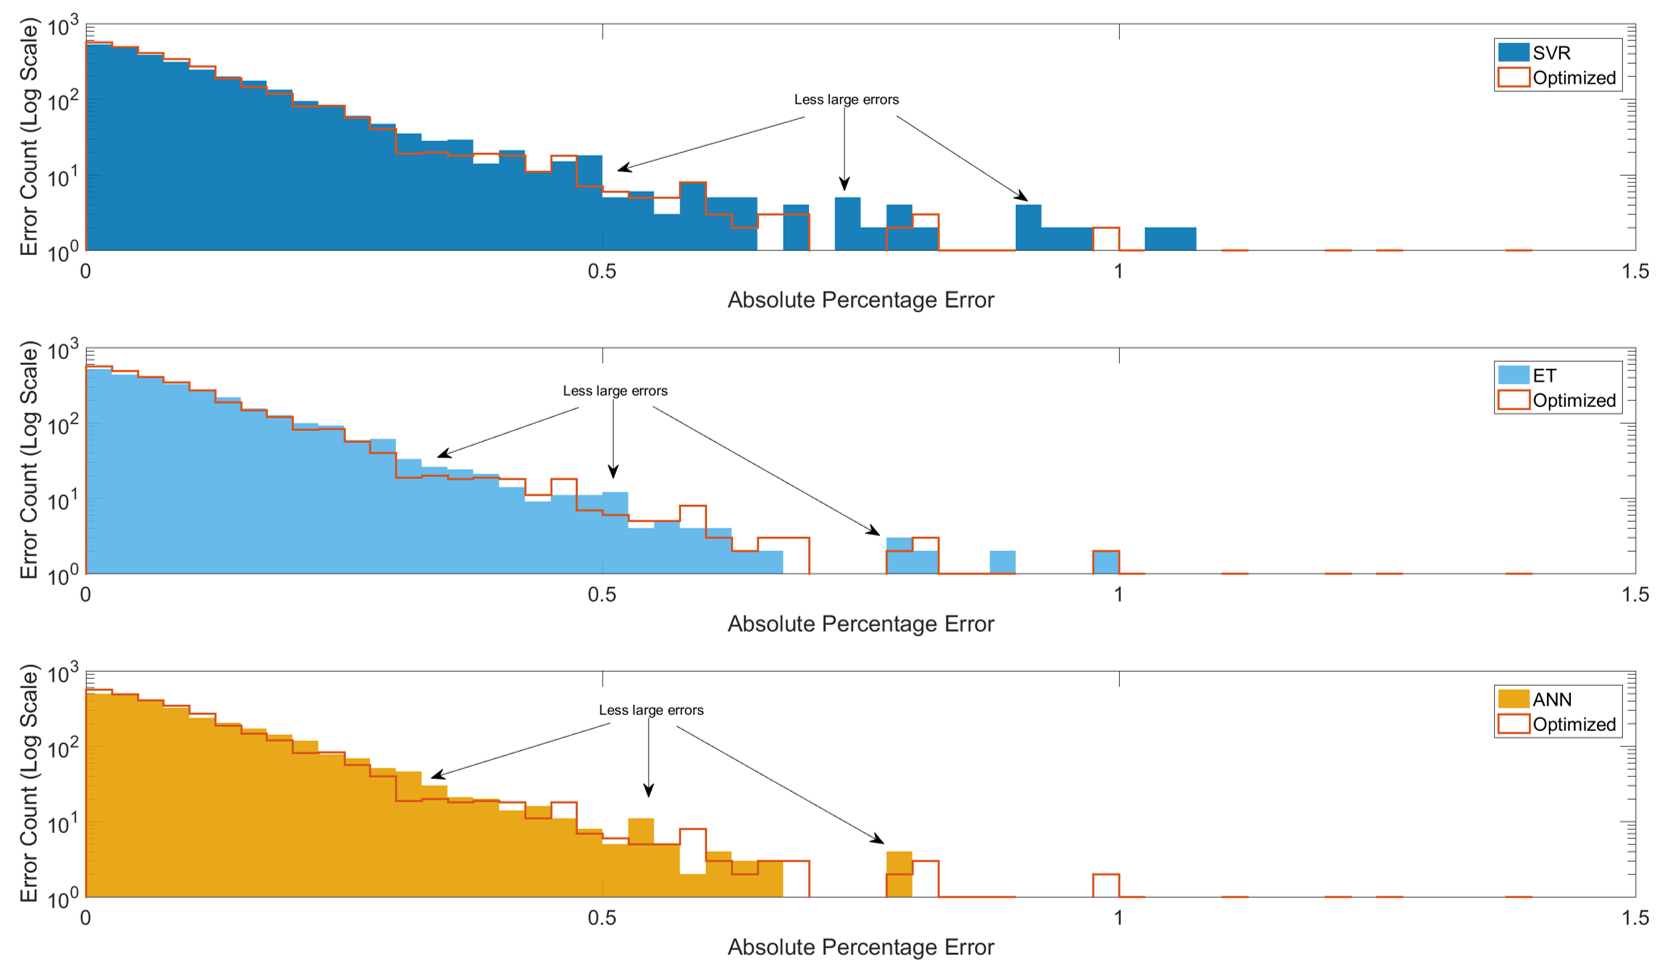
\includegraphics[width=88mm]{apecomparison}
 	\caption{Error Histogram of SVR, ET and ANN as compared to the optimized model}
 	\vspace{-0.3cm}
 	\label{errorhist}
 \end{figure}
\section{Conclusion}\label{conc}
The flexibility of air-conditioning load enables it to play a crucial role in demand response programs. To understand how AC load changes with various parameters in our test bed, we employed a discovery process that showed that for our case, the 15-min ahead AC load forecast do not depend much on exogenous weather conditions. A selection of variables were used to build forecasting models with SVMs, ETs and ANNs, and the best model for each technique is selected to be further investigated. Each of the selected models have different learning rates. ET takes the lead by reaching the minimum error rate after training on a week's worth of data, while ANN and SVM require 10 weeks and 12 weeks respectively. A customized linear combination technique was developed to mesh the three models, improving the accuracy above each selected model, to 0.1127.  
Based on our findings, future work will be on the following aspects. The first is to train the models on more data, as well as tune model parameters improvements in accuracy. The second is to integrate the system into an automated demand response agent, minimizing the power consumption of households with regards to price signals, while taking into account human comfort levels.

\section*{Acknowledgement}
This is work is supported in part by the Singapore GBIC R\&D grant NRF2015ENC-GBICRD001-028, and in part by the SUTD-MIT International Design Centre (IDC; idc.sutd.edu.sg).


\small
\bibliographystyle{IEEEtran}
\bibliography{ref_ac2} \footnotesize



% that's all folks
\end{document}


